
\section{十进制分解质因数}

\subsection{题目要求}

用户以十六进制输入一个自然数 $N(2 \le N \le 65528)$,程序需要将从 $N$ 开始的连续 8 个自然数都分解质因数。

经过了上一题的整个设计和开发流程之后,我们来做这道题就会显得比较简单。其中主要的分解质因数的步骤我们已经在上一题中实现过,因此在这一题中我们只需要实现简单的十六进制输入输出即可。

此外,由于上一题中我们已经实现了大部分 32 位无符号整数的运算,因此我们可以非常轻松地将本题的合法数据范围扩大到 $2 \le N \le 2^{32}-1$ 的范围内。

\subsection{关键部分程序流程图}

\subsubsection{十六进制输入}

\begin{figure}
  \centering
  \begin{tikzpicture}[node distance=2cm]
    \node (start) [startstop] {开始};
    \node (proc1) [process, below of=start] {$x \leftarrow 0$};
    \node (dec1)  [decision, below of=proc1, yshift=-1.5cm] {字符串是否读完};
    \node (proc2) [process, below of=dec1, yshift=-1.5cm] {令 $c$ 为当前字符};
    \node (dec2)  [decision, below of=proc2, yshift=-1cm] {$c$ 是否合法};
    \node (proc3) [process, below of=dec2, yshift=-1cm] {$x \leftarrow x \times 16$ \\ $x \leftarrow x + H(c)$};
    \node (proc4) [process, below of=proc3] {移动到字符串下一个字符};
    \node (echar) [io, right of=dec2, xshift=2.5cm] {输出错误:输入字符不合法};
    \node (stop)  [startstop, right of=proc3, xshift=2.5cm] {结束程序};
    \node (retn)  [startstop, right of=dec1, xshift=2.5cm] {返回结果 $x$};

    \draw [arrow] (start) -- (proc1);
    \draw [arrow] (proc1) -- (dec1);
    \draw [arrow] (dec1)  -- node[anchor=east] {No} (proc2);
    \draw [arrow] (dec1)  -- node[anchor=south] {Yes} (retn);
    \draw [arrow] (proc2) -- (dec2);
    \draw [arrow] (dec2)  -- node[anchor=east] {Yes} (proc3);
    \draw [arrow] (dec2)  -- node[anchor=south] {No} (echar);
    \draw [arrow] (proc3) -- (proc4);
    \node (p1) [shape=coordinate, left of=proc4, xshift=-1.5cm] {};
    \draw (proc4) -- (p1);
    \draw [arrow] (p1) |- (dec1);
    \draw [arrow] (echar) -- (stop);
  \end{tikzpicture}
  \caption{将字符串转化为无符号整数的流程图}
  \label{fig:r32hex}
\end{figure}

十六进制的输入相比十进制的输入大致相同,只不过我们需要将判断字符是否合法和最后乘的进制数做一些略微的修改。具体的实现过程可以参考图 \ref{fig:r32hex},其中出现的 $H(c)$ 函数是将字符 $c$ 转换为对应的十六进制下数字的函数。

对于 ASCII 码下,我们有

$$
H(c) = \begin{cases}
  c - 48, &48 \le c \le 57 \\
  c - 55, &65 \le c \le 70 \\
  c - 87, &97 \le c \le 102 \\
\end{cases}
$$

\subsubsection{十六进制输出}

\begin{figure}
  \centering
  \begin{tikzpicture}[node distance=2cm]
    \node (start) [startstop] {开始};
    \node (oxx) [io, below of=start] {输出前缀 0x};
    \node (prepare) [process, below of=oxx] {$z \leftarrow 0$ \\ $i \leftarrow 8$};
    \node (dec1) [decision, below of=prepare] {$i > 0$};
    \node (proc1) [process, below of=dec1] {$x \leftarrow x \lll 4$ \\ $c \leftarrow x \bmod 16$};
    \node (dec2) [decision, below of=proc1, yshift=-1cm] {$z = 0 \land c = 0$};
    \node (onum) [io, below of=dec2, yshift=-1cm] {输出 $H^{-1}(c)$};
    \node (proc3) [process, below of=onum] {$z \leftarrow 1$};
    \node (proc4) [process, below of=proc3] {$i \leftarrow i - 1$};
    \node (stop) [startstop, below of=proc4] {结束};

    \draw [arrow] (start) -- (oxx);
    \draw [arrow] (oxx) -- (prepare);
    \draw [arrow] (prepare) -- (dec1); 
    \draw [arrow] (dec1) -- node[anchor=east] {Yes} (proc1);
    \draw [arrow] (proc1) -- (dec2);

    \node (p1) [shape=coordinate, left of=dec2, xshift=-1.5cm] {};

    \draw (dec2) -- node[anchor=south] {Yes} (p1);
    \draw [arrow] (dec2) -- node[anchor=east] {No} (onum);
    \draw [arrow] (onum) -- (proc3);
    \draw [arrow] (proc3) -- (proc4);
    \draw [arrow] (p1) |- (proc4);

    \node (p2) [shape=coordinate, right of=proc4, xshift=2.5cm] {};
    \draw (proc4) -- (p2);
    \draw [arrow] (p2) |- (dec1);

    \node (p3) [shape=coordinate, left of=dec1, xshift=-2.5cm] {};
    \draw (dec1) -- node[anchor=south] {No} (p3);
    \draw [arrow] (p3) |- (stop);
  \end{tikzpicture}
  \caption{十六进制输出 32 位无符号数的流程图}
  \label{fig:w32hex}
\end{figure}

关于十六进制的输出过程我们虽然可以照搬十进制的输出,但其实我们有非常大的优化空间。由于计算机中的数字都是以二进制存放的,因此十六进制下的每一位都只是其二进制中的连续四位。因此我们可以直接使用循环移位来直接获取到十六进制下每一位的值。

另外需要注意的是前导 0 的问题,我们用一个标记来记录当前是否是前导零,并且避免无用的输出。具体输出的过程可以参考图 \ref{fig:w32hex},其中出现的 $x \lll 4$ 表示 $x$ 循环左移 4 位的操作,$H^{-1}(c)$ 函数用于将数字转换成对应的 ASCII 字符(使用大写字母),具体来说有

$$
H^{-1}(c) = \begin{cases}
  c + 48, &0 \le c \le 9 \\
  c + 55, &10 \le c \le 15 \\
\end{cases}
$$

\subsection{关键部分的源代码}

\subsubsection{以十六进制解析 32 位无符号数 r32hex}

\verb|r32hex| 子程序将会尝试以十六进制的方式解析用于输入的数字,如果解析失败则会调用 \verb|r32dec| 子程序再次尝试以十进制方式来解析用户输入的数字。读取的结果会直接写入到 \verb|BX| 寄存器保存的地址当中。

\begin{lstlisting}[language={[x86masm]Assembler},morekeywords={}]
r32hex  proc
        push    bp
        mov     bp, sp                  ; 保护环境
        mov     word ptr ss:[bx+2], 0   ; 初始化结果为 0
        mov     word ptr ss:[bx], 0
        cmp     rdstr[0], '0'           ; 检查第一个字符是否为 '0'
        jne     r32hexisnothex          ; 如果不是则尝试以十进制解析
        cmp     rdstr[1], 'x'           ; 检查第二个字符是否为 'x'
        jne     r32hexisnothex          ; 如果不是则尝试以十进制解析
r32hexishex:
        mov     si, 2                   ; SI 保存当前读入的字符下标
        mov     cx, 0                   ; CX 保存字符串长度
        mov     cl, strlen
        sub     cl, 2                   ; 需要循环的次数需要减去前导两个字符
        jcxz    r32hexreturn            ; 如果没有字符则直接结束
r32hexishexloop:
        mov     al, rdstr[si]           ; 将当前字符移动到 AL
        cmp     al, '0'                 ; 检查当前字符是否是数字
        jb      r32hexishexisnotdigit
        cmp     al, '9'
        ja      r32hexishexisnotdigit
        xor     al, 30h                 ; 如果是字符则减去 30h
        jmp     r32hexishexcontinue     ; 继续下一步运算
r32hexishexisnotdigit:
        cmp     al, 'a'                 ; 如果不是数字则检查是否是小写字母
        jb      r32hexishexisnotlower
        cmp     al, 'f'
        ja      r32hexishexisnotlower
        sub     al, 57h                 ; 如果是小写字母则减去 57h
        jmp     r32hexishexcontinue     ; 继续下一步运算
r32hexishexisnotlower:
        cmp     al, 'A'                 ; 如果依旧不是则检查是否是大写字母
        jb      r32hexishexisnotupper
        cmp     al, 'F'
        ja      r32hexishexisnotupper
        sub     al, 37h                 ; 如果是大写字母则减去 37h
        jmp     r32hexishexcontinue     ; 继续下一步运算
r32hexishexisnotupper:
        panic   einvch, 1               ; 如果都不是则字符非法,直接退出
r32hexishexcontinue:
        shl     word ptr ss:[bx], 1     ; 将 x 左移一位
        rcl     word ptr ss:[bx+2], 1
        shl     word ptr ss:[bx], 1     ; 将 x 左移一位
        rcl     word ptr ss:[bx+2], 1
        shl     word ptr ss:[bx], 1     ; 将 x 左移一位
        rcl     word ptr ss:[bx+2], 1
        shl     word ptr ss:[bx], 1     ; 将 x 左移一位
        rcl     word ptr ss:[bx+2], 1
        or      byte ptr ss:[bx], al    ; 将 x 加上读入的数字
        inc     si                      ; 移动到下一个字符
        loop    r32hexishexloop         ; 继续处理下一个字符
        jmp     r32hexreturn            ; 如果处理结束则返回
r32hexisnothex:
        call    r32dec                  ; 如果不是十六进制数则尝试以十进制解析
r32hexreturn:
        mov     sp, bp                  ; 恢复环境
        pop     bp
        ret                             ; 返回到原程序
r32hex  endp
\end{lstlisting}

\subsubsection{以十六进制打印 32 位无符号数 w32hex}

\verb|w32hex| 子程序用于将给定的 32 位无符号数以十六进制的方式输出,其中数据通过 \verb|BX| 寄存器给出内存地址。

\begin{lstlisting}[language={[x86masm]Assembler},morekeywords={}]
.data
wrtbuf  db      100 dup(0)              ; 输出缓冲区
hexstr  db      "0123456789ABCDEF"      ; 数字到字符的映射
.code
w32hex  proc
        push    di
        push    si
        push    ax
        push    cx
        push    dx                      ; 保护环境
        mov     wrtbuf[0], '0'          ; 将输出的第一个字符置 '0'
        mov     wrtbuf[1], 'x'          ; 将输出的第二个字符置 'x'
        mov     di, 2                   ; DI 保存当前字符串的长度
        mov     dl, 0                   ; DL = 0 表示当前应该舍去前导零
        mov     ax, ss:[bx+2]           ; 先处理数据的高 16 位
        mov     cx, 4                   ; 循环四次
w32hexloop1:
        rol     ax, 1                   ; AX 循环左移 4 次
        rol     ax, 1
        rol     ax, 1
        rol     ax, 1
        mov     si, ax                  ; SI 充当临时变量
        and     si, 0fh                 ; 取低的 4 位作为当前数位
        or      dx, si                  ; 将最低 4 位与 DL 取或
        test    dl, dl                  ; 检查 DL 是否为 0
        jz      w32hexloop1continue     ; 如果 DL = 0 则表示需要跳过前导零
        mov     dh, hexstr[si]          ; 通过 hexstr[si] 直接将数字转换成字符
        mov     wrtbuf[di], dh          ; 将字符写入到字符串末尾
        inc     di                      ; 字符串长度 ++
w32hexloop1continue:
        loop    w32hexloop1             ; 继续下位的处理
        mov     ax, ss:[bx]             ; 处理数据的低 16 位
        mov     cx, 4                   ; 循环四次
w32hexloop2:
        rol     ax, 1                   ; AX 循环左移 4 次
        rol     ax, 1
        rol     ax, 1
        rol     ax, 1
        mov     si, ax                  ; SI 充当临时变量
        and     si, 0fh                 ; 取最低的 4 位当作当前数位
        or      dx, si                  ; 将最低的 4 位与 DL 取或
        test    dl, dl                  ; 检查 DL 是否为 0
        jz      w32hexloop2continue     ; 如果 DL = 0 则表示要跳过前导零
        mov     dh, hexstr[si]          ; 通过 hexstr[si] 直接将数字转换成字符
        mov     wrtbuf[di], dh          ; 将字符写入到字符串末尾
        inc     di                      ; 字符串长度 ++
w32hexloop2continue:
        loop    w32hexloop2             ; 继续处理下一位
        cmp     di, 2                   ; 检查是否全都是前导零
        ja      w32hexskipaddzero       ; 如果不是则跳过下一步
        mov     wrtbuf[di], 30h         ; 如果是则主动输出一个 '0' 字符
        inc     di                      ; 字符串长度 ++
w32hexskipaddzero:
        mov     wrtbuf[di], 24h         ; 字符串末尾添加 '$' 字符
        print   wrtbuf                  ; 打印该字符串
        pop     dx                      ; 恢复环境
        pop     cx
        pop     ax
        pop     si
        pop     di
        ret                             ; 返回到原程序
w32hex  endp
\end{lstlisting}

此外我们额外提供一个 \verb|w16hex| 子程序用于输出 16 位的无符号数,同样也是在栈空间中将数据扩展成 32 位,然后直接调用 \verb|w32hex| 进行输出。数据通过 \verb|AX| 寄存器直接给出。

\begin{lstlisting}[language={[x86masm]Assembler},morekeywords={}]
w16hex  proc
        push    bp
        mov     bp, sp                  ; 保护环境
        sub     sp, 4                   ; 保留 4 字节
        mov     word ptr [bp-2], 0      ; 高位置零
        mov     word ptr [bp-4], ax     ; 低位复制
        lea     bx, [bp-4]              ; 给出 32 位数的地址
        call    w32hex                  ; 输出该数字
        mov     sp, bp                  ; 恢复环境
        pop     bp
        ret                             ; 返回到原程序
w16hex  endp
\end{lstlisting}

\subsubsection{主函数 \_start}

主函数 \verb|_start| 中主要实现读入数字,并且重复 8 次分解质因数并且将数字加一的操作。

\begin{lstlisting}[language={[x86masm]Assembler},morekeywords={}]
.data
prompt  db      "Input the starting number: ", "$"
.code
_start  proc
        mov     ax, @data               ; 给出数据段的地址
        mov     ds, ax                  ; 设置 DS 为数据段地址
        mov     es, ax                  ; 设置 ES 为数据段地址
        mov     bp, sp                  ; 设置 bp 为栈顶地址
        sub     sp, 4                   ; 保留 4 字节的空间,用于存放数据
        print   prompt                  ; 输出提示信息
        call    gets                    ; 读入一行字符
        lea     bx, [bp-4]              ; 给出结果保存的地址
        call    r32hex                  ; 以十六进制解析用户输入的数字
        cmp     word ptr [bp-2], 0      ; 检查 x > 1
        ja      continue                ; 如果 x > 1 则继续
        cmp     word ptr [bp-4], 1
        ja      continue                ; 如果 x > 1 则继续
        panic   enumsm, 1               ; 否则输出数字太小并结束程序
continue:
        mov     cx, 8                   ; 总共循环 8 次
plus1loop:
        lea     bx, [bp-4]              ; 给出操作数的地址
        call    factor                  ; 分解质因数
        add     word ptr [bp-4], 1      ; 将操作数 + 1
        adc     word ptr [bp-2], 0      ; 处理进位
        loop    plus1loop               ; 继续循环
        exit    0                       ; 结束程序
_start  endp

end     _start
\end{lstlisting}

其中值得注意的是 \verb|factor| 子程序大致与前一题的过程相同,只不过需要将 \verb|w32dec| 和 \verb|w16dec| 子程序都替换成同类的 \verb|w32hex| 和 \verb|w16hex| 子程序。

\subsection{运行结果及分析}

\begin{figure}
  \centering
  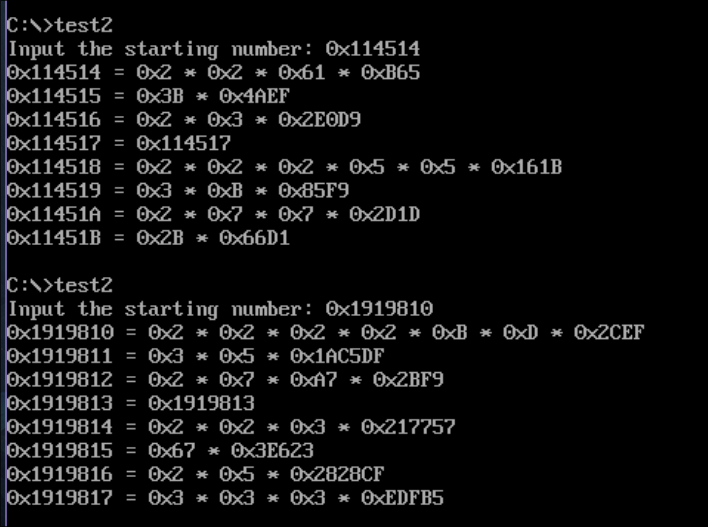
\includegraphics[width=300pt]{figure/test2res1.png}
  \caption{运行结果(a)}
  \label{fig:result2}
\end{figure}

从图 \ref{fig:result2} 中我们可以看出,程序可以正常地识别我们输入的十六进制数字,正确地将其分解质因数,并以十六进制的形式输出最终的结果。

\begin{figure}
  \centering
  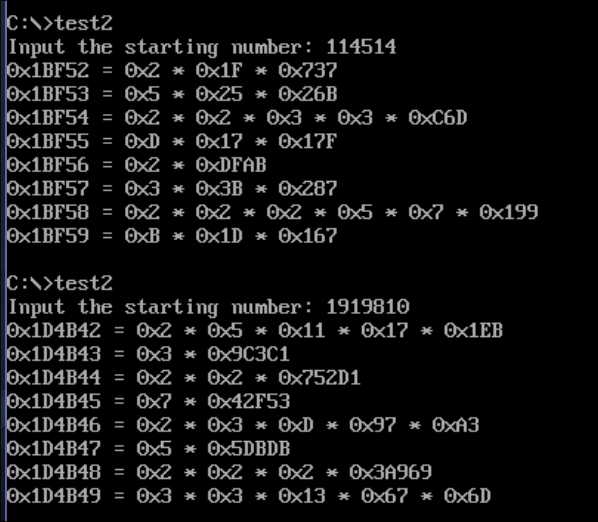
\includegraphics[width=300pt]{figure/test2res2.png}
  \caption{运行结果(b)}
  \label{fig:result3}
\end{figure}

从图 \ref{fig:result3} 中我们可以看出,程序在无法识别十六进制数据的时候会尝试以十进制的方式解析我们的输入内容,之后也可以正常处理输入的内容。

\begin{figure}
  \centering
  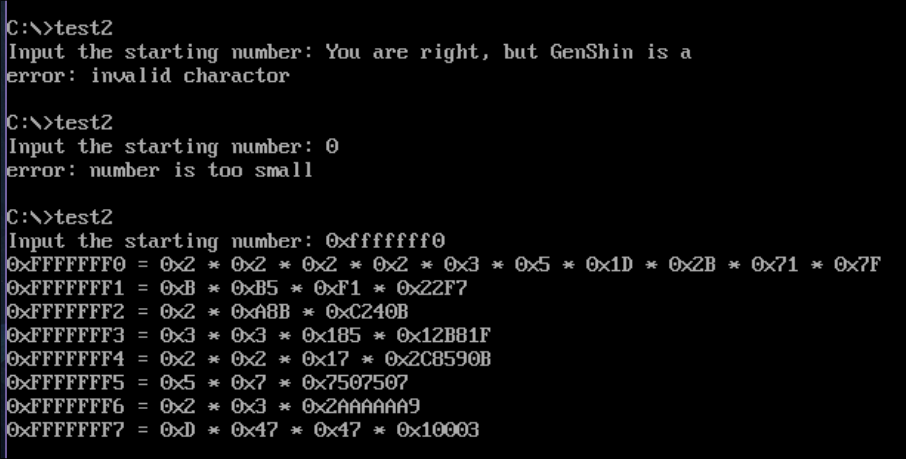
\includegraphics[width=300pt]{figure/test2res3.png}
  \caption{运行结果(c)}
  \label{fig:result4}
\end{figure}

从图 \ref{fig:result4} 中我们可以看出当用户输入了非法的内容之后可以正确地判断错误类型,并且也可以高效正确地处理极限数据的情况。

\subsection{遇到的问题及解决办法}

经过了前面一题的完整设计和实现之后再来实现本题就显得轻松许多,但是也有遇到一些新的问题。

首先 \verb|rol| 指令每次只能移动一个比特,或者使用 \verb|CL| 寄存器来存放移动的距离。但在文档中说如果给出的立即数大于 1,则会自动生成若干条重复的 \verb|rol xx, 1| 指令来进行填充,因为 8086 并没有对立即数大于 1 的情况进行编码。但在实际操作中发现编译器并不会主动展开对于立即数大于 1 的情况,而是会直接给出编译错误,这与文档中的预期行为有些许出入。

此外,在每次进入以 \verb|CX| 作为计数器的循环之前都使用 \verb|jcxz| 提前判断循环次数是否为 0 是一个比较重要的环节,不然当用户输入了特殊的内容使得 \verb|CX| 为 0 时便有可能导致程序陷入一个 $O(2^{16})$ 的循环,从而陷入错误的运算分支中。
